\chapter{Event Organizer Rules}

\section{Venue}

\oldrule{6d}
These are the guidelines by which Standard Skill competition is to be executed.
At times, however, situations may occur in which the regulations cannot be followed exactly.
This applies to minor details; not to principal rules.
For instance, if the size of the available accommodation would cause the size of the riding area to be slightly smaller than required, that can be approved by a majority vote of the judging panel.
Whatever differences from the rules are approved must be made known to all participants before competition.
Any situation that may occur for which the rules do not provide a solution, shall be solved by the Chief Judge or by a majority vote in a meeting chaired by the Chief Judge, at which all judges active in the concerned event must be present.

\subsection{Floor, Markings And Figure Shapes}
\oldrule{6.36}
See diagram.
The riding surface must allow flawless riding.
The riding area must be sufficiently illuminated.
An IUF representative will inspect the area to make sure it conforms to the requirements, and declare it ridable.
The surface of the riding floor must be clean, level, smooth and shall not be slippery.
Competition can be held on a floor that has not been declared ridable by the panel, but the results of such competition may not be officially recognized by the IUF, after investigation by the IUF rules committee.

\subsection{Riding Area Boundaries \label{subsec:freestyle_floor-markings-figure-shapes_riding-area-boundaries}}
\oldrule{6.36.1}
For international competitions, the outer boundaries must be 11 x 14 meters.
For other competitions, if space does not permit, the size may be smaller but will be no less than 9 x 12 meters.
All lines must be at least 3 cm wide and clearly marked, including the outer boundaries.

\begin{figure}[h]
\begin{center}
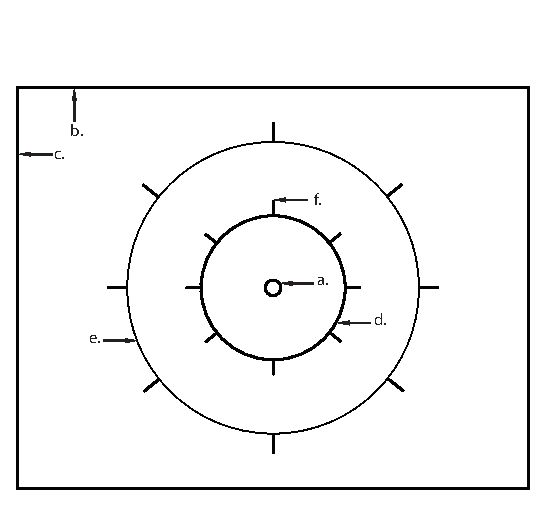
\includegraphics{std_skill_pattern_labeled}
\end{center}
\vspace{-20pt}
\caption{Riding Area Boundaries \label{fig:std_skill_pattern_labeled}}
\vspace{-10pt}
\end{figure}

\begin{enumerate}[a.]
\item Center circle (50 cm diameter)
\item Long edge of riding area (faces judges)
\item Short edge of riding area
\item Inner circle (4 m diameter) for circle figures
\item Outer circle (8 m diameter) for line and figure eights.
\item Quarter and diagonal circle marks (length 1 m) on the 4 m and 8 m circles.
Diagonals marked by going from corner to corner of the riding boundary.
\end{enumerate}

\section{Officials}

\begin{framed}
We only specified officials that are mentioned in the rules.
\end{framed}

\textbf{The host must designate the following officials for standard skill:
\begin{itemize}
\item Artistic Director
\item Chief Judge
\end{itemize}}

\section{Communication}

\begin{framed}
Some thoughts on additional required communication:
\begin{itemize}
\item the deadline for submission of the skills list
\item any changes to the standard rules
\item age groups
\item whether the performance space is non-standard
\end{itemize}
\end{framed}

\subsection{Announcing Of Results}

\oldrule{6.8}
Final results will be continuously announced and/or posted for public view.
Results Sheets will be posted after each age category of an event.
The protest period begins at this point.

\section{Age Groups}

\oldrule{6.31.1}
\textbf{The minimum age groups are} 0-14, 15-UP.
Best overall scores determine which competitors reach the Expert ranks.

\oldrule{6.2}
Riders are divided male/female in Standard Skill.

\section{Practice Space}

\begin{framed}
Is there a requirement for the host to provide practice time on the marked
floor?
\endframed}

\section{Media Types}
\oldrule{6.7.1}
The host is required to have the capability of playing recorded CDs.
Other media types may also be supported, at the host's discretion.
The Artistic Director is responsible for announcing what media types will be supported, and making sure the necessary equipment is provided.

\section{Music Volume}
\oldrule{6.7.3}
Volume level is controlled by the DJ, at instructions from the Chief Judge.
For Standard Skill, volume level should not be loud enough to interfere with judge communication, but otherwise similar to the level for Artistic Freestyle.
Some competitors' music may start with especially loud or quiet sections, and the DJ should be advised of these so volume levels do not get compensated in the wrong direction.
Some competitors may request that their music be played at lower levels.
These requests can be made directly to the DJ.
Requests for higher volumes must be approved by the Chief Judge, who has the option of passing this responsibility to the DJ.
